\newpage
\section{Analyse du potentiel des technologies libre dans le domaine de l'édition
vidéo et de leurs lacunes}

\paragraph{}
    Maintenant que les besoins et que les solutions existantes ont été
    analysées dans le détail on se doit de rendre compte de la situation
    actuel des technologies libres, de leurs communautés. Il est aussi
    important de chercher les raisons qui expliquent le fait que ces
    logiciels ne sont pas utilisés par les professionnels et trouver
    les solutions possibles qui permettrais de remédier à ce fait.

  \subsection{Etat de l'art}
      La création d'un logiciel open source d'édition vidéo, a
      été un objectif pour de nombreux projet logiciel. Du fait de
      la complexité inhérente au montage de vidéo de manière non
      linéaire, peu de projet ont pu durée afin de murir et être
      réellement utilisable par les utilisateurs comme le montre schéma suivant:
      \begin{figure}[!htbp]
          \begin{center}
              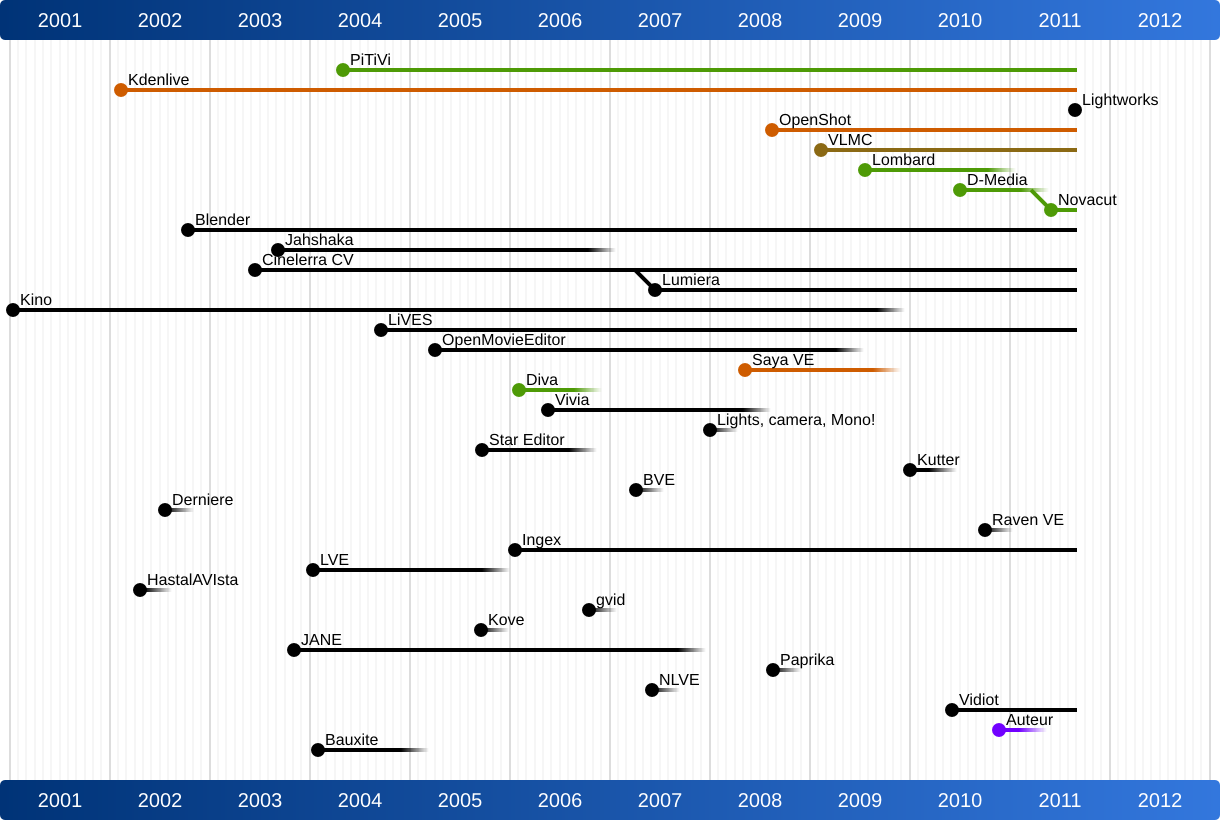
\includegraphics[width=0.9\textwidth]{images/open-source-video-editor-timeline}
          \end{center}
          \caption{Open source video editors timeline}
          \label{Yes}
      \end{figure}

      A l'heure actuel, il existe un nombre réduit de projet qui sont
      plus ou moins mature, mais des projet issue du monde propriétaire
      sont en train de faire la transition vers la libération de leur
      code. \cite{XXXXXXXXX}.

    \paragraph{}
      Mais il est plus intéressant d'analyser les frameworks d'édition
      vidéo  que les logiciels en tant que tel puisque toute la partie
      complexe de la tache est réalisé par ce composant.

  \subsection{Technologies}
    \subsubsection{Analyse technique}
    \subsubsection{Analyse des communauté}
  \subsection{Lacunes}
  \subsection{Solution possibles}

